% !TeX spellcheck = en_US
\section{Problem 5}


\begin{wrapfigure}{r}{0.45\textwidth}
	\centering
	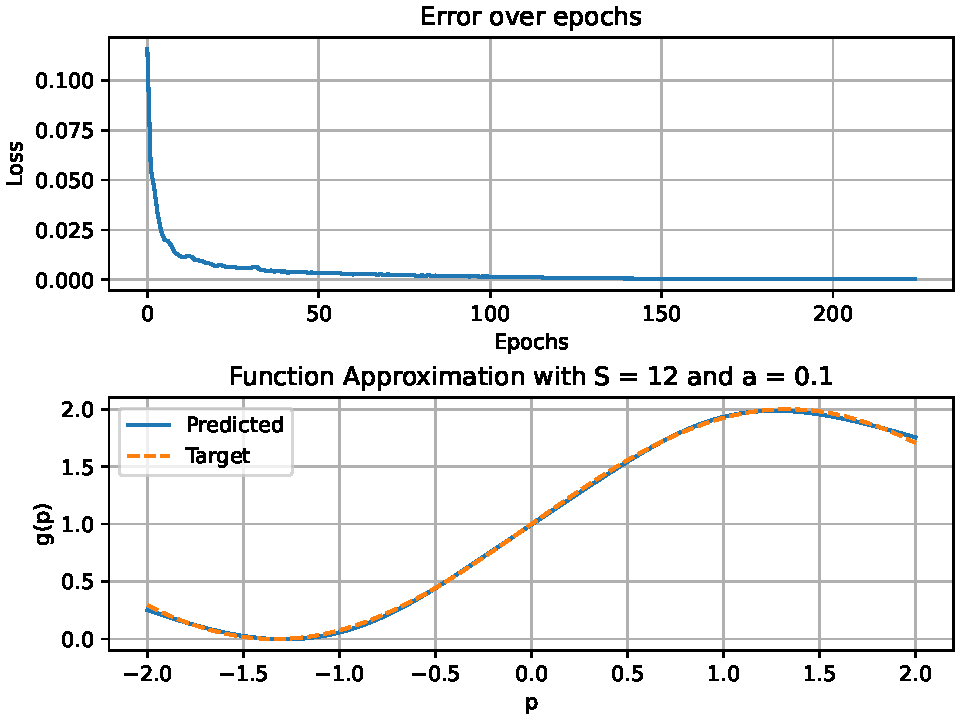
\includegraphics[width=0.43\textwidth]{../Problem 5/nn_1_12_1_nodp.pdf}
	\caption{Approximated function and error over iters}
	\label{fig:prob5_1_12_1_nodp}
\end{wrapfigure}

This problem relies on the parametric neural network from the previous problem, only that this time we have $S^1=12$ and learning rate $\alpha=0.1$. Despite the use of MATLAB programming language in Problem 4, this time we opted to use python-TensorFlow.\\

Looking at figure~\ref{fig:prob5_1_12_1_nodp}, we can clearly see that there's no difference between it and figure~\ref{fig:prob4_1-12-1_error_output}. This means that we're on the same level as before (\textit{same constraints, weight and bias initialization etc.}) and we can continue on this problem.
The code for this is located at \verb|Problem 5/keras_backprop.py|.\\

In order for us to not have unnecessary computations, we implemented \verb|Early Stopping|. This is a method that stops neural network's train if there's not a significant change in approximation error.